\documentclass[11pt]{article}
\usepackage{geometry}                % See geometry.pdf to learn the layout options. There are lots.

%\geometry{letterpaper}
\geometry{a4paper}

%\geometry{landscape}                % Activate for for rotated page geometry
%\usepackage[parfill]{parskip}    % Activate to begin paragraphs with an empty line rather than an indent
%\usepackage{graphicx}


%for dot2tex
\usepackage[pdftex]{graphicx}
%\usepackage{graphviz}
\usepackage{dot2texi}
\usepackage{pgf}
%\usepackage{tikz}  % commented for compilation (is it needed??)
%\usetikzlibrary{shapes,arrows,automata}  % commented for compilation (is it needed??)

\usepackage{amssymb}
\usepackage{color}
\usepackage{epstopdf}
\usepackage{listings}
\usepackage{textcomp}

 \usepackage[colorlinks=true, pdfstartview=FitV, linkcolor=blue,  citecolor=blue, urlcolor=blue]{hyperref}


\usepackage{sectsty}
%\allsectionsfont{\usefont{OT1}{phv}{bc}{n}\selectfont}
%\allsectionsfont{\sf\bf}
\allsectionsfont{\usefont{OT1}{phv}{bc}{w}\selectfont}


\DeclareGraphicsRule{.tif}{png}{.png}{`convert #1 `dirname #1`/`basename #1 .tif`.png}

\title{RooStats User's Guide}
\author{Kyle Cranmer, Lorenzo Moneta, Gr\eacute;gory Schott, Wouter Verkerke}
%\date{}                                           % Activate to display a given date or no date

\definecolor{listinggray}{gray}{0.9}
\definecolor{shellcommand}{rgb}{0.99,0.98,0.52}
\definecolor{lbcolor}{rgb}{0.98,0.98,0.98}
\lstset{
	backgroundcolor=\color{lbcolor},
	tabsize=4,
	rulecolor=,
	language=C++,
        basicstyle=\ttfamily\scriptsize,
%        upquote=true,                       % commented for compilation (is it needed??)
        aboveskip={1.5\baselineskip},
        columns=fixed,
        showstringspaces=false,
        extendedchars=true,
        breaklines=true,
        prebreak = \raisebox{0ex}[0ex][0ex]{\ensuremath{\hookleftarrow}},
        frame=single,
        showtabs=false,
        showspaces=false,
        showstringspaces=false,
        identifierstyle=\ttfamily,
        keywordstyle=\ttfamily\color[rgb]{0,0,1},
        commentstyle=\ttfamily\color[rgb]{0.133,0.545,0.133},
        stringstyle=\ttfamily\color[rgb]{0.627,0.126,0.941},
}

%%%%%%%%%%%%%%%%%%%%%%%%%%%%%%%%%%%%%%%
%%%%%%%%%%%%%%%%%%%%%%%%%%%%%%%%%%%%%%%
\begin{document}
\sf

{\flushright 
Document version 0 

\flushright 
\today

}

\vspace{2in}

\hrule
\vspace{.1in}
{\huge RooStats}
\vspace{.5in}

{\huge User's Guide}
\vspace{.1in}
\hrule

\vspace{.5in}

{\large Kyle Cranmer, Gr\'egory Schott, Lorenzo Moneta, Wouter Verkerke}

\vspace{2in}
{\em With contributions from:}\\

Kevin Belasco, Danilo Piparo, Giacinto Piacquadio, Maurizio Pierini, George H. Lewis, Alfio Lazzaro, Mario Pelliccioni, Matthias Wolf


%%%%%%%%%%%%%%%%%%%%%%%%%%%%%%%%%%%%%%
%%%%%%%%%%%%%%%%%%%%%%%%%%%%%%%%%%%%%%%
\newpage
\tableofcontents 

%%%%%%%%%%%%%%%%%%%%%%%%%%%%%%%%%%%%%%
%%%%%%%%%%%%%%%%%%%%%%%%%%%%%%%%%%%%%%%
%\newpage
%\begin{abstract}
%Abstract
%\end{abstract}




%%%%%%%%%%%%%%%%%%%%%%%%%%%%%%%%%%%%%%
%%%%%%%%%%%%%%%%%%%%%%%%%%%%%%%%%%%%%%%
\newpage
\section{Introduction}

The RooStats project aims to provide a comprehensive, flexible, and validated suite of statistical tools within ROOT.  Early on in the project it was decided to leverage the data modeling approach developed in RooFit, which is already well-established within high-energy physics and beyond.  Thus, RooStats can be seen as providing high-level statistical tools, while RooFit provides the core data modeling language as well as many low-level aspects of the functionality.   In the ongoing process of developing RooStats, RooFit is also undergoing rapid development.

One of the major goals of RooStats is to provide a unified framework for different statistical methods.  Early on in the project it was demonstrated that RooFit is well suited for the three major types of statistical inference:
\begin{description}
 \item[Classical / Frequentist] This ``school'' of statistics restricts itself to making statements of the form ``probability of the data given the hypothesis''.  The definition of probability in this context is based on a limit of frequencies of various outcomes.  In that sense it is objective.
 \item[Bayesian] This ``school'' of statistics allows one to make statements of the form "probability of the hypothesis given the data", which requires a prior probability of the hypothesis.  Often the definition of probability in this context is a ``degree of belief''.  
 \item[Likelihood-based] This intermediate approach does not require a prior for the hypothesis, but also is not guaranteed to poses the properties that frequentists methods aim to achieve (or achieve by construction).  These approaches do ``obey the likelihood principle'' (as do Bayesian methods), while frequentist methods do not. 
\end{description}
The developers of RooStats appreciate that there are many different approaches to answering the same types of problems.  There are pros and cons of various techniques, and we aim to provide a framework which can accommodate any of them.

{\flushleft \textbf{One Model, Many Methods}}

A common scenario that we hope to address with RooStats is the comparison of different statistical approaches for the same statistical problem.  Without a unified framework, these comparisons are complicated by the fact that each method must: a) re-create the model (eg. probability density function(s) for the data) and b) represent the data itself.  Having redundant modeling and data representation is error prone and often complicates the comparison (or makes it practically impossible).\footnote{Of course, these types of cross-checks can also be very useful! }  In that sense, RooStats aims to be like TMVA\footnote{The Toolkit for MultiVariate Analysis is also distributed in ROOT \url{http://tmva.sourceforge.net}.}, providing utilities to easily try and compare multiple statistical techniques.  By relieving the technical overhead associated to these types of comparisons, the hard work can go into improved modeling of the problem at hand and asking better questions.

{\flushleft \textbf{Types of Statistical Questions}}

One of the first steps in any statistical analysis is to carefully pose the question that one wishes to answer.  Most of these questions can be classified as follows:
\begin{description}
 \item[Parameter Estimation] Find the most likely (`best fit') values of the parameters of a model given data.
 \item[Hypothesis Testing] Based on the data accept or reject a given hypothesis.  Often one tests a null hypothesis against an alternative.  When the hypothesis has no free parameters it is called `simple' and when it has free parameters it is called `composite'.
 \item[Confidence intervals] Find a region in the parameter space that is consistent with the data.  In the frequentist setting, one desires for this interval or region to `cover' the true parameter point with a specified probability (or confidence).  In the Bayesian setting, one wishes for the interval or region to contain some fixed amount of the posterior probability.
 \item[Goodness of Fit] Quantify how well a model fits the data, without reference to an alternative.
\end{description}
RooStats provides tools for each of these broad class of questions in addition to some miscellaneous utilities.  The design of the software is explicitly organized around these broad classes of questions: for instance the interface \texttt{IntervalCalculator} is common to all tools that produce \texttt{ConfidenceInterval}s. 

{\flushleft \textbf{Combining Results \& Digital Publishing}}

Combining results from multiple experiments in order to enhance sensitivity of a measurement or improve the power of a hypothesis test is common.  The challenge of combining results is primarily logistical, since a proper combination requires low-level information from each experiment be brought together to form one large statistical test. Again, this is hindered by the fact that the ingredients to the combination are heterogeneous (eg. different formats, technologies, and conventions).  

The major advancement that was made by the RooStats project is the concept of the \textit{workspace}.   The power of the workspace is that it allows one to save data and an arbitrarily complicated model to disk in a ROOT file.  These files can then be shared or archived, and they provide all the low-level ingredients necessary for a proper combination in a unified framework.   The \texttt{ RooWorkspace} provides this low-level functionality, thus it is technically part of RooFit (along with its documentation and several tutorial macros).

This form of digital publishing has great potential, consider a few examples: It allows for one to publish likelihood functions in $n$-dimensions instead of resorting to 2-dimensional contours.  It allows for one to interface the likelihood function to even higher-level software packages (eg. extraction of fundamental lagrangian parameters from experimental measurements).  It allows for one to generate toy data for the observables given any parameter point, which is necessary for a truly frequentist calculation.  It allows for combinations with other experiments as already mentioned.

%%%%%%%%%%%%%%%%%%%%%%%%%%%%%%%%%%%%%%
\subsection{Getting Started}

Since December 2008, RooStats has been distributed in the ROOT release since version 5.22 (December 2008).  To use RooStats, you need a version of ROOT greater than 5.22, but you will probably want the most recent ROOT version since the project is developing quickly.  

{\flushleft \textbf{Option 1) Download the binaries for the latest ROOT release}}

You can download the most recent version of ROOT here: \url{http://root.cern.ch/}

{\flushleft \textbf{Option 2) Check out and build the ROOT trunk}}

If you prefer to build ROOT from source, 
\begin{lstlisting}[backgroundcolor=\color{shellcommand}]
svn co http://root.cern.ch/svn/root/trunk root
\end{lstlisting}
then build and install ROOT via (you may want different configure options)
\begin{lstlisting}[backgroundcolor=\color{shellcommand}]
configure --enable-roofit
make
make install 
\end{lstlisting}


{\flushleft \textbf{Option 3) Check out and build the RooStats branch}}

If you need a development or bug-fix that is not yet in a ROOT release, you can download the most recent version of the code from ROOT's subversion repository.  To check it out, go to some temporary directory and type:
\begin{lstlisting}[backgroundcolor=\color{shellcommand}]
 svn co https://root.cern.ch/svn/root/branches/dev/roostats root
\end{lstlisting}
then build and install ROOT via (you may want different configure options)
\begin{lstlisting}[backgroundcolor=\color{shellcommand}]
configure --enable-roofit
make
make install 
\end{lstlisting}

\vspace{.2in}

For more information about building ROOT from source, see the ROOT webpage:\\ \url{http://root.cern.ch/drupal/content/installing-root-source}.  

\newpage
%%%%%%%%%%%%%%%%%%%%%%%%%%%%%%%%%%%%%%
\subsection{Other Resources}

{\flushleft The RooStats Web Page}:\\
\url{https://twiki.cern.ch/twiki/bin/view/RooStats/}

{\flushleft The Root User's Guide}:\\
\url{http://root.cern.ch/drupal/content/users-guide}

{\flushleft The RooFit User's Guide:}\\
\url{ftp://root.cern.ch/root/doc/RooFit_Users_Manual_2.91-33.pdf}

{\flushleft RooFit Tutorials}:\\
 \url{http://root.cern.ch/root/html/tutorials/roofit/} 
 
{\flushleft RooStats Tutorials}:\\
 \url{http://root.cern.ch/root/html/tutorials/roostats/} 


%%%%%%%%%%%%%%%%%%%%%%%%%%%%%%%%%%%%%%
%\subsection{Goals of the RooStats Project}

%%%%%%%%%%%%%%%%%%%%%%%%%%%%%%%%%%%%%%
%\subsection{Relationship to RooFit}


%%%%%%%%%%%%%%%%%%%%%%%%%%%%%%%%%%%%%%
\subsection{Terminology used in this guide}

\begin{description}
\item[ model ] a probability density function that describes some observables.  We use the term model for both parametric models (eg. a Gaussian is parametrized by a mean and standard deviation) and non-parametric models (eg. histograms or KEYS pdfs).

\item[ observable(s)] quantities that are directly measured by an experiment and present in a data set.  The distribution of the observables are predicted by the model.  Models are normalized such that the integral of the model over the observables is 1.

\item[ auxiliary observable] observables that are come from an auxiliary experiment (eg. a control sample or a preceding experiment).

\item[ parameter of interest] quantities used to parametrize a model that are `interesting' in the sense that one wishes to estimate their values,  place limits on them, etc (eg. masses, cross-sections, and the like).

\item[ nuisance parameter ] quantities used to parametrize a model that are uncertain but not `interesting' in the above sense (eg. background normalization, shape parameters associated to systematic uncertainties, etc.)

\item[ control sample ] a data set independent of the main measurement (defining auxiliary observables) often used to constrain nuisance parameters by simultaneous considering it together with the main measurement.0

\end{description}

%%%%%%%%%%%%%%%%%%%%%%%%%%%%%%%%%%%%%%
\subsection{Types of Statistical Tools in RooStats}

\begin{figure}[htbp]
\begin{center}
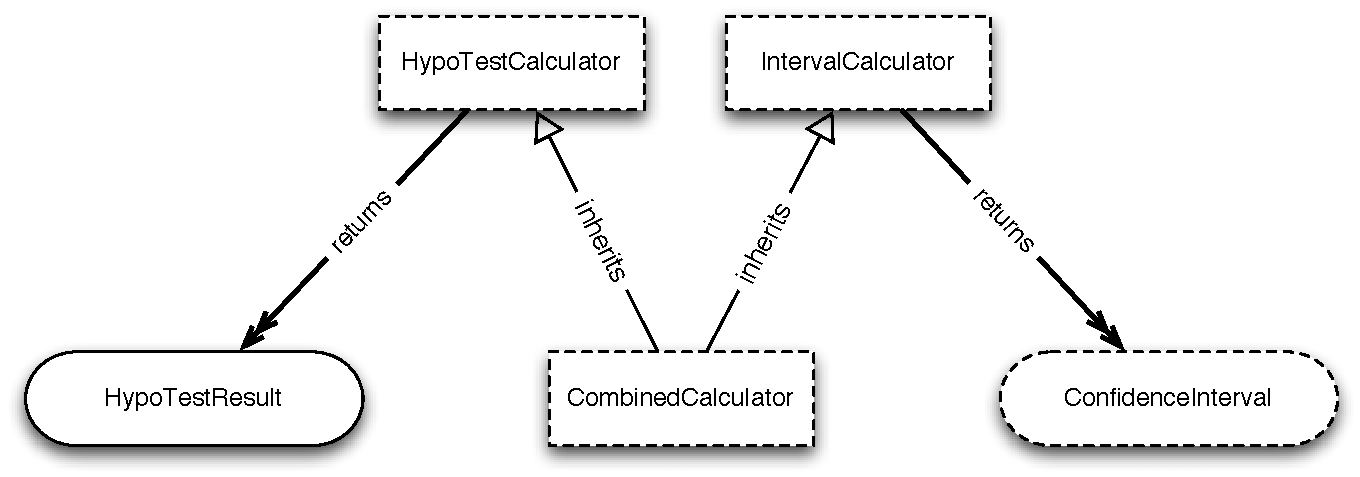
\includegraphics[width=\textwidth]{RooStats_OverviewOfInterfaces.pdf}
\caption{An class diagram of the interfaces for hypothesis testing and confidence interval calculations.  The diagram shows the classes used to return the results of these statistical tests as well.}
\label{fig:OverviewOfInterfaces}
\end{center}
\end{figure}



%%%%%%%%%%%%%%%%%%%%%%%%%%%%%%%%%%%%%%
\subsection{Design Philosophy: Mapping Mathematics to Software}

Mathematical representation:
\[
  G(x|\mu, \sigma)
\]

Representation in RooFit / RooStats code:
  
\lstinputlisting{GaussianModel.C}

Graphical Representation 

\begin{figure}[htb]
  \begin{picture}(500, 100)(0,0)
\begin{dot2tex}[dot, options=-tmath,autosize,graphstyle={scale=0.8,transform shape}]
  \input{GaussianModel.dot}
 \end{dot2tex} 
\end{picture}
\caption{test}
\end{figure}

%\begin{figure}[htb]
%\lstinputlisting{GaussianModel2.C}
%\caption{code }
%\end{figure}

%Graphical Representation 

%\begin{figure}[htb]
%  \begin{picture}(500, 100)(0,0)
%\begin{dot2tex}[dot, options=-traw,autosize,graphstyle={scale=0.8,transform shape}]
%  \input{GaussianModel2.dot}
% \end{dot2tex} 
%\end{picture}
%\caption{test}
%\end{figure}

%%%%%%%%%%%%%%%%%%%%%%%%%%%%%%%%%%%%%%
%%%%%%%%%%%%%%%%%%%%%%%%%%%%%%%%%%%%%%
\section{Parameter Estimation}

Parameter estimation, or `point estimation' is the general class of statistical tests in which one wishes to estimate the value of some parameter $\theta$ given some data $x$ and a model $P(x|\theta)$.  In high energy physics, this is usually referred to as ``fitting'', and the estimate that is given is usually the ``maximum likelihood estimate'' (MLE).  The most common tool for providing maximum likelihood estimates in high energy physics is \textsc{minuit}.

In general an \textit{estimator} for $\theta$ can be denoted $\hat{\theta}(x)$ and it has an expected value $E[\hat{\theta}]$.  If the expectation value of the estimator is equal to the true value of the parameter, then the estimator is called \textit{unbiased}.   The \textit{variance} of the estimator is $var[\hat\theta] = E[ (\hat\theta - E[\hat\theta])^2]$.  

Two naturally desirable properties of estimators are for them to be unbiased and have minimal mean squared error (MSE). These cannot in general both be satisfied simultaneously: a biased estimator may have lower mean squared error (MSE) than any unbiased estimator: despite having bias, the estimator variance may be sufficiently smaller than that of any unbiased estimator, and it may be preferable to use, despite the bias; see estimator bias~[Wikipedia].

Among unbiased estimators, there often exists one with the lowest variance, called the minimum variance unbiased estimator (MVUE). In some cases an unbiased efficient estimator exists, which, in addition to having the lowest variance among unbiased estimators, satisfies the Cram\'er-Rao bound, which is an absolute lower bound on variance for statistics of a variable~[Wikipedia].

RooFit provides a general interface to determine the MLE for all probability density functions via: \texttt{RooAbsPdf::fitTo(RooAbsData\& data,...)}.  It is possible to use other minimization algorithms other than \textsc{minuit}, which is outlined in the RooFit documentation.

Currently, RooStats does not provide functionality for point estimation beyond what is found directly in RooFit.  However, RooStats does offer significantly more options when one wants to consider frequentist confidence intervals or Bayesian credible intervals on the parameters.

%%%%%%%%%%%%%%%%%%%%%%%%%%%%%%%%%%%%%%
%%%%%%%%%%%%%%%%%%%%%%%%%%%%%%%%%%%%%%
\section{Test Statistics and Sampling Distributions}

A \textit{test statistic} $T(x)$ is a general term for a numerical summary of the data.  Typically a test statistic is a single number, though it can be have multiple components.  Usually a test statistic is best thought of as a mapping of the data to a real number, and that mapping often depends on the values of the parameters of a model (implicit in the notation $T(x)$.  

For instance, for simple hypothesis testing the Neyman-Pearson lemma states that the likelihood ratio is the most powerful test statistic for testing a null hypothesis against an alternative.  In a simple number counting experiment, the number of events usually serves as the test statistic.  In more complicated cases one might use the profile likelihood ratio as the test statistic to summarize the preference of the data toward one hypothesis or the other.  As will be described below, RooStats provides a general interface and several implementations for the notion of a test statistic.

Note, a \textit{sufficient statistic} is a statistic which has the property of sufficiency with respect to a statistical model and its associated unknown parameter, meaning that "no other statistic which can be calculated from the same sample provides any additional information as to the value of the parameter".  In most situations relevant for high energy physics, the only distributions in the exponential family have sufficient statistics.

A \textit{sampling distribution} is very familiar to high energy physicists, it is the distribution for some quantity that one obtains from sampling some parent distribution $n$ times.  It is most commonly the result of Monte Carlo sampling, and often obtained from ``toy Monte Carlo'' or ``pseudo-experiments''.  In statistical tests, it is common to build the sampling distribution for some test statistic $T$ by first using Monte Carlo techniques to sample $x$ from $P(x|\theta)$ and then evaluating the test statistic $T(x)$.  There are other techniques for building these sampling distributions.



\begin{figure}[htbp]
\begin{center}
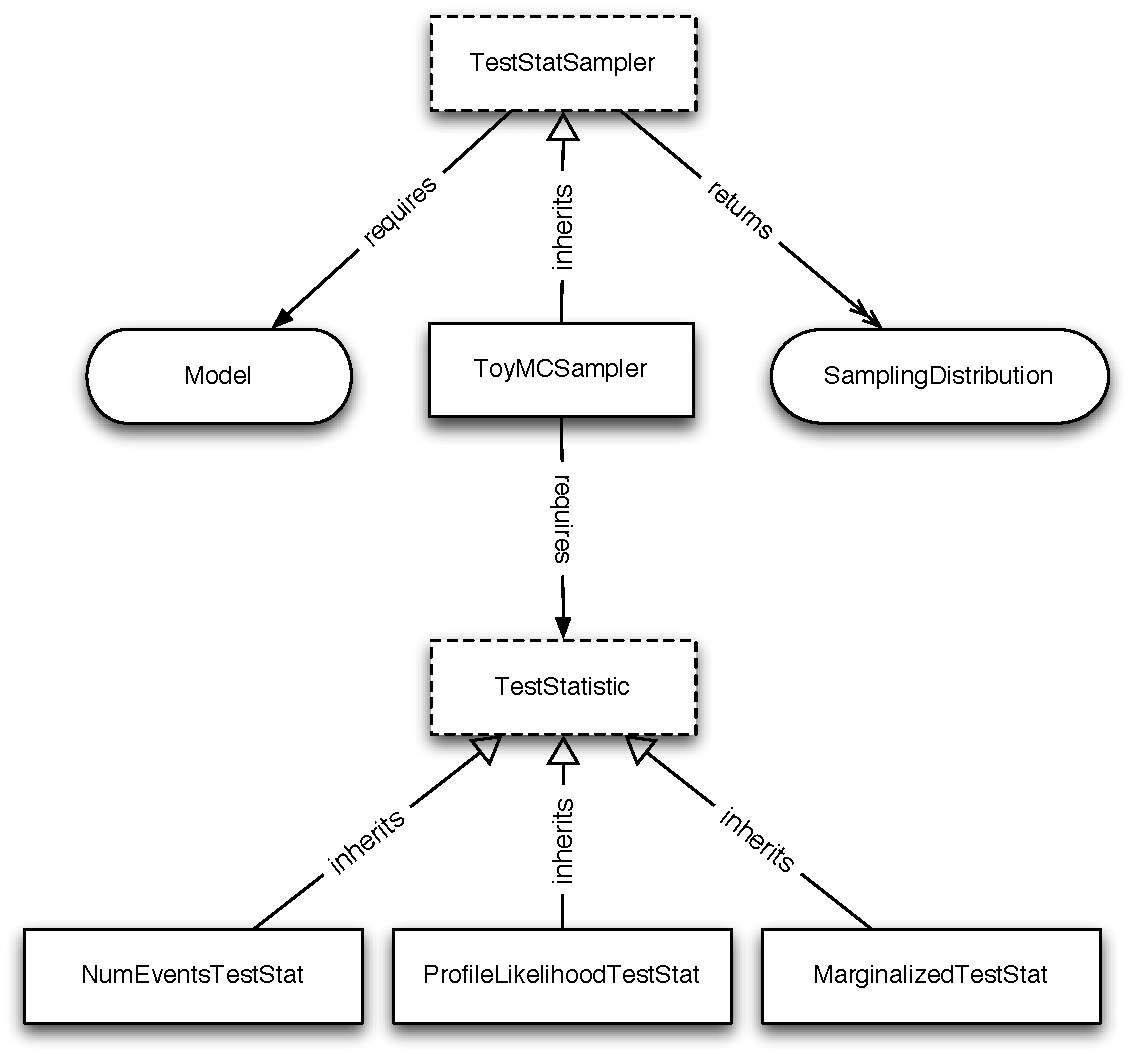
\includegraphics[width=\textwidth]{RooStats_TestStatistic.pdf}
\caption{Class diagram showing the relationship between the interface classes TestStatSamler and TestStatistic.  The diagram shows a few concrete implementations of the TestStatistic interface and the TestStatSampler interface.}
\label{fig:TestStatistic}
\end{center}
\end{figure}

%%%%%%%%%%%%%%%%%%%%%%%%%%%%%%%%%%%%%%
	\subsection{TestStatistic interface and implementations}


We added a new interface class called TestStatistic. It defines the method \texttt{Evaluate(data, parameterPoint)}, which returns a double.  This class can be used in conjunction with the ToyMCSampler class to generate sampling distributions for a user-defined test statistic.  

The following concrete implementations of the TestStatistic interface are currently available

ProfileLikelihoodTestStatReturns the log of profile likelihood ratio.  Generally a powerful test statistic.
NumEventsTestStatReturns the number of events in the dataset.  Useful for number counting experiments.
DebuggingTestStat Simply returns a uniform random number between 0,1.  Useful for debugging.
SamplingDistribution and the TestStatSampler interface and implementations

We introduced a ``result'' or data model class called SamplingDistribution, which holds the sampling distribution of an arbitrary real valued test statistic.  The class also can return the inverse of the cumulative distribution function (with or without interpolation).  

We introduced an interface for any tool that can produce a SamplingDistribution, called TestStatSampler.  The interface is essentially GetSamplingDistribution(parameterPoint) which returns a SamplingDistribution based on a given probability density function.  We foresee a few versions of this tool based on toy Monte Carlo, importance sampling, Fourier transforms, etc.  The following concrete implementation of the TestStatSampler interface are currently available

ToyMCSampler uses a Toy Monte Carlo approach to build the sampling distribution.  The pdf's generate method to generate is used to generate toy data, and then the test statistic is evaluated at the requested parameter point.
DebuggingSampler Simply returns a uniform distribution between 0,1.  Useful for debugging.
NeymanConstruction and FeldmanCousins

A flexible framework for the Neyman Construction was added in this release. The NeymanConstruction is a concrete implementation of the IntervalCalculator interface, but it needs several additional components to be specified before use. The design factorizes the choice of the parameter points to be tested, the choice of the test statistic, and the generation of sampling distribution into separate parts (described above).  Finally, the NeymanConstruction class is simply in charge of using these parts (strategies) and constructing the confidence belt and confidence intervals.  The ConfidenceBelt class is still under development, but the current version works fine for producing ConfidenceIntervals.  We are also working to make this class work with parallelization approaches, which is not yet complete.

The FeldmanCousins class is a separate concrete implementation of the IntervalCalculator interface.  It uses the NeymanConstruction internally, and enforces specific choices of the test statistic and ordering principle to realize the Unified intervals described by Feldman and Cousins in their paper Phys.Rev.D57:3873-3889,1998.

%%%%%%%%%%%%%%%%%%%%%%%%%%%%%%%%%%%%%%
%%%%%%%%%%%%%%%%%%%%%%%%%%%%%%%%%%%%%%
\section{Hypothesis Testing}

Hypothesis testing is one of the most common procedures in science.  In \textit{simple hypothesis testing} one considers a null hypothesis $H_0$ and an alternate hypothesis $H_1$, both of which are completely specified and provide models for the data.  

Define: Type I \& Type II errors, size, and power.

The Neyman-Pearson lemma states that the likelihood ratio $P(x|H_1)/P(x|H_0)$ provides the most powerful test statistic for testing the alternate against the null.  This is the basis for the ubiquity of the use of teh likelihood ratio; however, it is only the most powerful test in this very limited situation.

More commonly one does not have a fully specified simple hypothesis, but a \textit{composite hypothesis} $P(x|\mu,\nu)$ that is parametrized.  It may be parametrized according to some parameter of interest $\mu$ (e.g., the mass of a particle) or by some nuisance parameter $\nu$ (e.g., an unknown background rate).  In these cases, the Neyman-Pearson lemma is not applicable.  One would like to find a test statistic that is most powerful over the full range of $\mu$ -- which is referred to as Uniformly Most Powerful (UMP).  Unfortunately, UMP tests don't exist in general.  

There is a precise dictionary that relates hypothesis tests to confidence intervals.  In fact, the frequentist method for deriving confidence intervals is referred to as an ``inverted hypothesis test''.

In RooStats we wish to support several different techniques for hypothesis testing.  They mainly differ in the way that they incorporate systematic effects.  There are only very few cases in which hypothesis tests with systematics has a clear ``solution'' from first principles.  In a more general setting the field has developed several techniques, and new ones are being advocated given recent interaction with the professional statistics community.  Some of the techniques included in RooStats are mainly avaialbe for consistency with historical practice in the field.

As denoted in Fig.~\ref{fig:OverviewOfInterfaces}, the interface for tools that peform hypothesis tests in RooStats is called \texttt{HypoTestCalculator}.  After configuring a HypoTestCalculator, one simply requests the result via \texttt{HypoTestCalculator::GetHypoTest()}.

Below we describe three concrete implementatons.

%%%%%%%%%%%%%%%%%%%%%%%%%%%%%%%%%%%%%%
	\subsection{Single Channel Number Counting with Background Uncertainty}

Here we describe the ratio of Poisson means.

%%%%%%%%%%%%%%%%%%%%%%%%%%%%%%%%%%%%%%
	\subsection{Profile Likelihood Ratio (the method of MINOS)}

The approximate frequentist method based on Wilks' theorem.





%%%%%%%%%%%%%%%%%%%%%%%%%%%%%%%%%%%%%%
	\subsection{The Hybrid Calculator}

This is the traditional frequentist ToyMC method; however, because of
its Bayesian marginalization of nuisance parameters it is not purely
frequentist.  Hence the technique is often referred to as a
``Bayesian-Frequentist Hybrid''.
 We define $H_b$ as the hypothesis that no signal is
present over the background and $H_{sb}$ the hypothesis that signal is
also present. In order to quantify the degree in which each hypotheses
are favoured or excluded by the experimental observation one chooses a
test-statistics which ranks the possible experimental outcomes. A
commonly used test statistics consist as the ratio of the likelihood
function in both hypotheses: $Q=L_{sb}/L_b$ and the quantity $-2\ln Q$
may also be used instead of $Q$. The HybridCalculator class of RooStats provides alternative
choices for the test statistics such as the number of events or the
profiled likelihood ratio.


A comparison of $Q_\mathrm{obs}$ for the data being tested to the
probability distributions $dP/dQ$ expected in both hypotheses allows
to compute the confidence levels:
\begin{eqnarray}
  CL_{sb} = P_{sb}(Q<Q_\mathrm{obs}), & \mathrm{where} & P_{sb}(Q<Q_\mathrm{obs}) = \int_{-\infty}^{Q_\mathrm{obs}}\frac{dP_{sb}}{dQ} dQ, \\
  CL_{b} = P_{b}(Q<Q_\mathrm{obs}), & \mathrm{where} & P_{b}(Q<Q_\mathrm{obs}) = \int_{-\infty}^{Q_\mathrm{obs}}\frac{dP_{b}}{dQ} dQ.
\end{eqnarray}
Small values of $CL_{sb}$ (resp.~$CL_{b}$) point out poor compatibility with the $H_{sb}$ (resp.~$H_{b}$)
hypothesis and favour the $H_{b}$ (resp.~$H_{s}$) hypothesis.
The functional form of the $dP_{sb}/dQ$ and $dP_{b}/dQ$ pdfs not being
known a priori, a large amount of toy Monte-Carlo experiments are performed
in order to determine it for
two families of pseudo datasets: the ones in the signal+background and the ones in 
the background-only hypothesis (see figure~\ref{m2lnQ}).


\begin{figure}[h]
    \begin{center}
%%        \includegraphics[width=87mm]{figures/m2lnQsample.png}
        \caption{The distributions of $-2\ln Q$ in the background-only
                 (red, on the right) and signal+background (blue,
                 on the left) hypotheses. The black line represents
                 the value of $-2\ln Q$ on the tested data.  The
                 shaded areas represent $1-CL_{b}$ (red) and $CL_{sb}$
                 (blue).\label{m2lnQ}}
    \end{center}
\end{figure}

A significance estimation can be obtained using formula~\ref{nsigmasfromCL2} on
$CL_{sb}$. Moreover, the tested data can be said to be excluded at a
given CL if $1-CL_{sb}$ is smaller than this CL (or alternatively the
$CL_s$ prescription can be used (see below)). By varying the
hypothesis being tested (for example varying the signal cross-section
as on figures~\ref{htautau_lim_1}, \ref{htautau_lim_2}, \ref{hww_lim}
and \ref{combination_plot}) one may also scan for the type of model
that can be excluded with the given data.
It should be observed that these confidence intervals do not have the
same meaning as the ones obtained with the profile likelihood method
or the Bayesian credibility intervals.
\par
Systematics uncertainties are taken into account  using Bayesian
Monte-Carlo sampling.
For each toy Monte-Carlo experiment the effective value 
of the nuisance parameters is varied before generating the toy Monte-Carlo sample itself 
(that includes in addition the Poisson fluctuations).
The whole phase space of the nuisance parameters is thus sampled through
Monte-Carlo integration. The final net effect consist in a broadening
of the $-\ln Q$ distribution and thus, as expected in presence of
systematic uncertainties, a degraded separation of the hypotheses.


%%%%%%%%%%%%%%%%%%%%%%%%%%%%%%%%%%%%%%
%%%%%%%%%%%%%%%%%%%%%%%%%%%%%%%%%%%%%%
\section{Confidence Intervals}

%%%%%%%%%%%%%%%%%%%%%%%%%%%%%%%%%%%%%%
	\subsection{Profile Likelihood Ratio (the method of MINOS)}

Suppose we have, for each of $N$ events in a collection, a set of
measured quantities \mbox{$\underline{x}=(x_a,\,x_b,\,x_c,\,\ldots)$}
whose distributions are described by a joint probability density
function, or pdf, $f(\underline{x},\underline{\theta})$, where
$\underline{\theta}=(\theta_1,\,\theta_2,\,\theta_3,\,\ldots )$ is a
set of $K$ parameters. The likelihood function is then defined by
the equation:
\begin{equation}
    \label{likelihood}
    L(\underline{x},\underline{\theta})=\prod^{N}_{i=1}f({\underline{x}}_{i},\underline{\theta}).
\end{equation}
To ease the calculations, the negative of the logarithm of the likelihood
function $-\ln{L}$ (negative log-likelihood) is often used.

Focussing on a one-dimensional case, the profile likelihood method
requires to perform a scan over a sensible range of values of the
parameter of interest $\theta_{0}$. For every point of this scan, the
value of $\theta_{0}$ is fixed and $-\ln{L(\theta_{0})}$ is minimised
(i.e.~a fit is performed) with respect to the remaining $K-1$
parameters. The maximum likelihood estimator of the $\theta_{0}$
parameter, noted $\hat{\theta}_0$, is the value where the negative
log-likelihood function is at its minimum
$-\ln{L(\hat{\theta}_0)}$. 

Figure~\ref{plscan} shows an example of a profiled negative
log-likelihood curve which has been offset by
$-\ln{L(\hat{\theta}_0)}$. From this construction, it is possible to
easily obtain the one- or two-sided confidence interval we are
interested in. In the assumption of a parabolic shape of the negative
log-likelihood function\footnote{It can be shown that this approach is
also valid for a general scan shape \cite{Metzger}.}, the boundaries
of a confidence intervals correspond to the values of
$\theta_0$ with
\begin{equation}
    \label{parabolicnll}
    \Delta nll = -(\ln{L(\theta_0)}-\ln{L(\hat{\theta}_0)}) = \frac{n_\sigma^{2}}{2},\ \mathrm{with}\ n_\sigma=\frac{\theta_{0}-\hat{\theta}_{0}}{\sigma}.
\end{equation}
where $\sigma$ represent the Gaussian standard deviations. The mapping between the desired 
confidence level (CL) and the value of $n_\sigma$ is given, in the Gaussian assumption, by the formulae:
\begin{eqnarray}
    \label{nsigmasfromCL1}
    &n_\sigma = \sqrt{2}\cdot \mathrm{Erf}^{-1}(CL) & \mathrm{(two-sided)} \\
    &n_\sigma = \sqrt{2}\cdot \mathrm{Erf}^{-1}(2 \cdot CL -1) & \mathrm{(one-sided)}
    \label{nsigmasfromCL2}
\end{eqnarray}
where $\mathrm{Erf}^{-1}$ is the Gaussian inverse error function. In
the later case, an upper limit on the parameter $\theta_0$ would then
correspond then to the value $\theta_0>\hat{\theta}_0$ obeying
equations~\ref{parabolicnll} and~\ref{nsigmasfromCL2}.



%%%%%%%%%%%%%%%%%%%%%%%%%%%%%%%%%%%%%%
	\subsection{Neyman Construction}

This is the general class for performing a NeymanConstruction.
Some details in the TestStatsitic section, more to come.

%%%%%%%%%%%%%%%%%%%%%%%%%%%%%%%%%%%%%%
	\subsection{Feldman-Cousins}

This is a light weight class that encodes a specific configuration of the more general purpose  Neyman Construction class.

%%%%%%%%%%%%%%%%%%%%%%%%%%%%%%%%%%%%%%
	\subsection{Neyman Construction with nuisance parameters}

%%%%%%%%%%%%%%%%%%%%%%%%%%%%%%%%%%%%%%
	\subsection{The ``Profile Construction''}

%%%%%%%%%%%%%%%%%%%%%%%%%%%%%%%%%%%%%%
	\subsection{Markov Chain Monte Carlo}

	Another way to determine a confidence interval for parameters is to use Markov Chain Monte-Carlo with the MCMCCalculator.  Like the other IntervalCalculator derived classes, once you initialize and configure your MCMCCalculator, just call GetInterval(), which returns an MCMCInterval (ConfInterval derived class).
	
	\subsubsection{MCMCCalculator}
	\label{sec:MCMCCalculator}
	
	MCMCCalculator runs the Metropolis-Hastings algorithm (section \ref{sec:MetropolisHastings}) with the parameters of your model, a $-log($Likelihood$)$ function constructed from the model and data set, and a ProposalFunction (section \ref{sec:ProposalFunction}).  This generates a Markov chain posterior sampling, which is used to create an MCMCInterval (section \ref{sec:MCMCInterval}).
	
	The most basic usage of an MCMCCalculator is automatically set up with the simplified 3-arg constructor (or 4-arg with RooWorkspace).  This automatic configuration package consists of  a UniformProposal, 10,000 Metropolis-Hastings iterations, 40 burn-in steps, and 50 bins for each RooRealVar; it also determines the interval by kernel-estimation, turns on sparse histogram mode, and finds a 95\% confidence interval (see sections \ref{sec:MetropolisHastings} and \ref{sec:MCMCInterval} to learn about these options).  These are reasonable settings designed to minimize configuration steps and hassle for beginning users, making the code very simple:
	
	\lstinputlisting{mcmc_examples/mcmc-most-basic.C}
	
	All other MCMCCalculator constructors are designed for maximum user control and thus do not have any automatic settings.  You can customize the configuration (and override any automatic settings) through the mutator methods provided by MCMCCalculator.  It may be easiest to use the default no-args constructor and perform all configuration with these methods.
	
	\lstinputlisting{mcmc_examples/mcmc-custom-config.C}
	
	\subsubsection{ProposalFunction}
	\label{sec:ProposalFunction}
	The ProposalFunction interface generalizes the task of proposing points in some distribution for some set of variables, presumably for use with the Metropolis-Hastings algorithm.
	
	PdfProposal is the most powerful and general ProposalFunction derived class.  It proposes points in the distribution of any RooAbsPdf you pass it to serve as its proposal density function.  It also provides a generalized means of updating PDF parameters based on the current values of PDF observables.  This is useful for centering the proposal density function around the current point when proposing others or for advanced control over the widths of peaks or anything else in the proposal function.  It also has a cacheing mechanism (off by default) which almost always significantly speeds up proposals.
	
	Here's a PdfProposal construction example that uses a covariance matrix from the RooFitResult.  Be careful that your RooArgLists have the same order of variables as the covariance matrix uses:
	
	\lstinputlisting{mcmc_examples/mcmc-pdfproposal.C}
	
	Since PdfProposal functions are powerful but annoying to build, we created ProposalHelper to make it easier.  It will build a multi-variate Gaussian proposal function and has some handy options for doing so.  Here's how to create exactly the same proposal function as in the example above.  Note that using RooFitResult::floatParsFinal() to set the RooArgList of variables ensures the right order.
	
	\lstinputlisting{mcmc_examples/mcmc-proposalhelper.C}
	
	ProposalHelper can also create a PdfProposal with a "Bank of Clues" (cite paper) component.  This will add a PDF with a kernel placed at each "clue" point to the proposal density function.  This will increase the frequency of proposals in the clue regions which can be especially useful for helping the Metropolis-Hastings algorithm find small and/or distant regions of interest (no free lunch, of course, you need to know these regions beforehand to pick the clue points).  Just pass a RooDataSet with (possibly weighted) entries for each clue point.  You can also choose what fraction of the total proposal function integral comes from the bank of clues PDF.
	
	\lstinputlisting{mcmc_examples/mcmc-proposalhelper-clues.C}
	
	Using the covariance matrix from a RooFitResult is not required.  If you do not set the covariance matrix, ProposalHelper constructs a pretty good default for you -- a diagonal matrix with sigmas set to some fraction of the range of each corresponding RooRealVar.  You can set this fraction yourself (the default is 1/6th).
	
	To help Metropolis-Hastings find small and/or distant regions of interest that you do not know beforehand, you can set ProposalHelper to add a fraction of uniform proposal density to the proposal function.  Use the ProposalHelper::SetUniformFraction() method to choose what fraction the uniform PDF makes up of the entire proposal function integral.

	UniformProposal is a specialized implementation of a ProposalFunction that proposes points in a uniform distribution over the range of the variables.  Its low overhead as compared to a PdfProposal using a RooUniform PDF and guaranteed symmetry makes it much faster at proposing in a purely uniform distribution.  UniformProposal does not need a cacheing mechanism.
	
	\subsubsection{MetropolisHastings}
	\label{sec:MetropolisHastings}
	A MetropolisHastings object runs the Metropolis-Hastings algorithm to construct a Markov chain posterior sampling of a function.  At each step in the algorithm, a new point is proposed (section \ref{sec:ProposalFunction}) and possibly "visited" based on its likelihood relative to the current point.  Even when the proposal density function is not symmetric, MetropolisHastings maintains detailed balance when constructing the Markov chain by counterbalancing the relative likelihood between the two points with the relative proposal density.  That is, given the current point $x$, proposed point $x'$, likelihood function $L$, and proposal density function $Q$, we visit $x'$ iff
	\begin{center}
	$\displaystyle \frac{L(x')}{L(x)} \frac{Q(x | x')}{Q(x' | x)} \geq Rand[0,1]$
	\end{center}
	MetropolisHastings supports ordinary and log-scale functions.  This is particularly useful for handling either regular likelihood or $\pm$log-likelihood functions.  You must tell MetropolisHastings the type and sign of function the you have supplied (if you supply a regular function, make sure that it is never 0).  Then set a ProposalFunction, parameters to propose for, and a number of algorithm iterations.  Call ConstructChain() to get the Markov chain.
	
	\lstinputlisting{mcmc_examples/mcmc-metropolishastings-regular.C}
	
	Here's how to do a similar task using a negative log-likelihood function instead:
	
	\lstinputlisting{mcmc_examples/mcmc-metropolishastings-nll.C}
	
	\subsubsection{MCMCInterval}
	\label{sec:MCMCInterval}
	MCMCInterval is a ConfInterval that determines the confidence interval on your parameters from a MarkovChain (section \ref{sec:MarkovChain}) generated by Monte Carlo.  To determine the confidence interval, MCMCInterval integrates the posterior where it is the tallest until it finds the correct cutoff height $C$ to give the target confidence level $P$.  That is, to find
	\begin{center}
	$\displaystyle \int\limits_{f(\mathbf{x}) \, \ge \, C} f(\mathbf{x}) \,d^nx = P$
	\end{center}
	MCMCInterval has a few methods for representing the posterior to do this integration.  The default is simply as a histogram, so this integral turns into a summation of bin heights.  If you have no more than 3 parameters and 100 bins, a standard histogram will be fine.  However, for higher dimensions or bin numbers, it is faster and less memory intensive to use a sparse histogram data structure (aside: in a regular histogram, 4 variables with 100 bins each requires $\sim$4GB of contiguous memory, a tall order).  By default, the histogram method adds bins to the interval until at least the desired confidence level has been reached (use MCMCInterval::SetHistStrict() to change this).
	
	Another posterior representation option is kernel-estimation (often termed "keys") using a RooNDKeysPdf, which has more theoretical validity because it takes the arbitrariness out of choosing a histogram binning.  The kernel-estimation method usually takes longer than the histogram method because it typically requires several integrations to find the right cutoff such that $|P_{calculated} - P_{target}| < \epsilon$ ($\epsilon = 0.01$ by default).
	
	To try to remove the arbitrariness of the starting point in the Markov chain, which was rather random when it was generated by MetropolisHastings, a certain number of "burn-in" steps can be ignored from the beginning of the chain.  Generally it is a good idea to use burn-in, but the number of steps to discard depends on the function you are sampling and your proposal function, so it is off by default.  Usually you will tell the MCMCCalculator (section \ref{sec:MCMCCalculator}) the number of burn-in steps to use by calling MCMCCalculator::SetNumBurnInSteps(), since it configures the MCMCInterval.  For future versions, automatic burn-in step calculations are being considered.
	
	\subsubsection{MCMCIntervalPlot}
	\label{sec:MCMCIntervalPlot}
	
	The MCMCIntervalPlot class helps you to visualize the interval and Markov chain.  The function MCMCIntervalPlot::Draw() will draw the interval as determined by the type of posterior representation the MCMCInterval was configured for (i.e. histogram or keys PDF).  To specifically ask for a certain interval determination to be drawn, use DrawHistInterval() or DrawKeysPdfInterval().
	
	\lstinputlisting{mcmc_examples/mcmc-mcmcintervalplot.C}
	
	\subsubsection{MarkovChain}
	\label{sec:MarkovChain}
	A MarkovChain stores a series of weighted steps through N-dimensional space in which each step depended only on the one before it.  Each step in the chain also has a $-log($likelihood$)$ value associated with it.  The class supplies some simple methods to access each step in the chain in order:
	
	\lstinputlisting{mcmc_examples/mcmc-markovchain.C}
	

%%%%%%%%%%%%%%%%%%%%%%%%%%%%%%%%%%%%%%
%%%%%%%%%%%%%%%%%%%%%%%%%%%%%%%%%%%%%%
\section{Goodness of Fit}

%%%%%%%%%%%%%%%%%%%%%%%%%%%%%%%%%%%%%%
%%%%%%%%%%%%%%%%%%%%%%%%%%%%%%%%%%%%%%
\section{Coverage Studies}

%%%%%%%%%%%%%%%%%%%%%%%%%%%%%%%%%%%%%%
%%%%%%%%%%%%%%%%%%%%%%%%%%%%%%%%%%%%%%
\section{Utilities}

%%%%%%%%%%%%%%%%%%%%%%%%%%%%%%%%%%%%%%
	\subsection{The Number Counting PDF Factory}

%%%%%%%%%%%%%%%%%%%%%%%%%%%%%%%%%%%%%%
	\subsection{RooStatsUtils}

		\subsubsection{Standalone number counting functions}

		\subsubsection{Converting between p-values and significance}

%%%%%%%%%%%%%%%%%%%%%%%%%%%%%%%%%%%%%%
	\subsection{SPlot}

This initial description of \texttt{RooStats::SPlot} is taken directly from the documentation of\\ \url{http://root.cern.ch/root/html/TSPlot.html}.  It mainly describes the method, which is common to both the RooStats implementation and \texttt{TSPlot}.  The main difference between the implementations is that the RooStats implementation allows one to use arbitrary models created with RooFit's data modeling language.

A common method used in High Energy Physics to perform measurements is
the maximum Likelihood method, exploiting discriminating variables to
disentangle signal from background. The crucial point for such an
analysis to be reliable is to use an exhaustive list of sources of
events combined with an accurate description of all the Probability
Density Functions (PDF).


To assess the validity of the fit, a convincing quality check
is to explore further the data sample by examining the distributions of
control variables. A control variable can be obtained for instance by
removing one of the discriminating variables before performing again
the maximum Likelihood fit: this removed variable is a control
variable. The expected distribution of this control variable, for
signal, is to be compared to the one extracted, for signal, from the
data sample. In order to be able to do so, one must be able to unfold
from the distribution of the whole data sample.


The TSPlot method allows to reconstruct the distributions for
the control variable, independently for each of the various sources of
events, without making use of any a priori knowledge on this
variable. The aim is thus to use the knowledge available for the
discriminating variables to infer the behaviour of the individual
sources of events with respect to the control variable.



TSPlot is optimal if the control variable is uncorrelated with the discriminating variables.




A detail description of the formalism itself, called 
 $\hbox{$_s$}{\cal P}lot$
 

M. Pivk and F. R. Le Diberder, Nucl. Inst. Meth. A (in press), physics/0402083




\subsubsection{The method}




The  $\hbox{$_s$}{\cal P}lot$ technique is developped in the above context of a maximum Likelihood method making use of discriminating variables.



One considers a data sample in which are merged several species
of events. These species represent various signal components and
background components which all together account for the data sample.
The different terms of the log-Likelihood are:

\begin{itemize}
 \item[$N$] the total number of events in the data sample,
 \item[${\rm N}_{\rm s}$] the number of species of events populating the data sample,
 \item[${\rm N}_{\rm i}$] the number of events expected on the average for the $i^{th}$ species,
 \item[${\rm f}_i(y_e)$] the value of the PDFs of the discriminating variables $y$ for the $i^{th}$ species and for event $e$, 
 \item[$x$] the set of control variables which, by definition, do not appear in the expression of the Likelihood function $L$
\end{itemize}

The extended log-Likelihood reads:
 \begin{equation}
{\cal L}=\sum_{e=1}^{N}\ln \Big\{ \sum_{i=1}^{{\rm N}_{\rm s}}N_i{\rm f}_i(y_e) \Big\} -\sum_{i=1}^{{\rm N}_{\rm s}}N_i ~.
\end{equation}

From this expression, after maximization of $L$ with respect to the $N_i$ parameters, a weight can be computed for every event and each species, in order to obtain later the true distribution  ${\hbox{\bf {M}}}_i(x)$ of variable $x$  If ${\rm n}$ is one of the 
 ${\rm N}_{\rm s}$ species present in the data sample, the weight for this species is defined by:



 \begin{equation}
\begin{Large}\fbox{$
{_s{\cal P}}_{\rm n}(y_e)={\sum_{j=1}^{{\rm N}_{\rm s}} \hbox{\bf V}_{{\rm n}j}{\rm f}_j(y_e)\over\sum_{k=1}^{{\rm N}_{\rm s}}N_k{\rm f}_k(y_e) } $}\end{Large} ~,
\end{equation}
 

where $\hbox{\bf V}_{{\rm n}j}$ is the covariance matrix resulting from the Likelihood maximization.
This matrix can be used directly from the fit, but this is numerically
less accurate than the direct computation:

 \begin{equation}
\hbox{\bf V}^{-1}_{{\rm n}j}~=~
{\partial^2(-{\cal L})\over\partial N_{\rm n}\partial N_j}~=~
\sum_{e=1}^N {{\rm f}_{\rm n}(y_e){\rm f}_j(y_e)\over(\sum_{k=1}^{{\rm N}_{\rm s}}N_k{\rm f}_k(y_e))^2} ~.
\end{equation}


The distribution of the control variable $x$ obtained by histogramming the weighted events reproduces, on average, the true distribution ${\hbox{\bf {M}}}_{\rm n}(x)$ .



The class TSPlot allows to reconstruct the true distribution 
${\hbox{\bf {M}}}_{\rm n}(x)$ of a control variable $x$ for each of the 
${\rm N}_{\rm s}$ species from the sole knowledge of the PDFs of the discriminating variables ${\rm f}_i(y)$  The plots obtained thanks to the TSPlot class are called 
 $\hbox{$_s$}{\cal P}lots$
 


\subsubsection{Some properties and checks}




Beside reproducing the true distribution, 
$\hbox {$_s$}{\cal P}lots$ bear remarkable properties:


Each $x$ distribution is properly normalized:
 \begin{equation}
\sum_{e=1}^{N} {_s{\cal P}}_{\rm n}(y_e)~=~N_{\rm n}~.
\end{equation}
 
For any event:

 \begin{equation}
\sum_{l=1}^{{\rm N}_{\rm s}} {_s{\cal P}}_l(y_e) ~=~1 ~.
\end{equation}

That is to say that, summing up the 
 ${\rm N}_{\rm s}$
$\hbox {$_s$}{\cal P}lots$  one recovers the data sample distribution in $x$  and summing up the number of events entering in a 
 $\hbox{$_s$}{\cal P}lot$
for a given species, one recovers the yield of the species, as provided by the fit.


 \begin{equation}
\sigma[N_{\rm n}\  _s\tilde{\rm M}_{\rm n}(x) {\delta x}]~=~\sqrt{\sum_{e \subset {\delta x}} ({_s{\cal P}}_{\rm n})^2} ~.
\end{equation}
 reproduces the statistical uncertainty on the yield  $N_{\rm n}$, as provided by the fit: 
$\sigma[N_{\rm n}]\equiv\sqrt{\hbox{\bf V}_{{\rm n}{\rm n}}}$ 
Because of that and since the determination of the yields is optimal
when obtained using a Likelihood fit, one can conclude that the
 $\hbox{$_s$}{\cal P}lot$
  technique is itself an optimal method to reconstruct distributions of control variables.



\begin{itemize}

\item A maximum Likelihood fit is performed to obtain the yields $N_i$ of the various species. 
The fit relies on discriminating variables $y$ uncorrelated with a control variable $x$ 
the later is therefore totally absent from the fit. 

 \item The weights ${_s{\cal P}}$ are calculated using Eq.~\ref{eq.} where the covariance matrix is taken from Minuit.

 \item Histograms of $x$ are filled by weighting the events with ${_s{\cal P}}$  

 \item Error bars per bin are given by Eq. \ref{eq:ErrorPerBin}. 
\end{itemize}

The $\hbox {$_s$}{\cal P}lots$ reproduce the true distributions of the species in the control variable $x$  within the above defined statistical uncertainties.





\subsection{Bernstein Correction}


BernsteinCorrection is a utility in RooStats to augment a nominal PDF with a polynomial  correction term.  This is useful for incorporating systematic variations to the nominal PDF.   The Bernstein basis polynomails are particularly appropriate because they are positive definite. 

This tool was inspired by the work of Glen Cowan together with Stephan Horner, Sascha Caron,  Eilam Gross, and others.   The initial implementation is independent work.  The major step forward in the approach was  to provide a well defined algorithm that specifies the order of polynomial to be included  in the correction.  This is an emperical algorithm, so in addition to the nominal model it  needs either a real data set or a simulated one.  In the early work, the nominal model was taken to be a histogram from Monte Carlo simulations, but in this implementation it is generalized to an arbitrary PDF (which includes a RooHistPdf).  The algorithm basically consists of a  hypothesis test of an nth-order correction (null) against a n+1-th order correction (alternate).  The quantity q = -2 log LR is used to determine whether the n+1-th order correction is a major  improvement to the n-th order correction.  The distribution of q is expected to be roughly  $\chi^2$ with one degree of freedom if the n-th order correction is a good model for the data.   Thus, one only moves to the n+1-th order correction of q is relatively large.  The chance that  one moves from the n-th to the n+1-th order correction when the n-th order correction  (eg. a type 1 error) is sufficient is given by the Prob($\chi^2_1 >$ threshold).  The constructor  of this class allows you to directly set this tolerance (in terms of probability that the n+1-th  term is added unnecessarily).


\section{Tutorials}


Several new tutorials were added for RooStats.  They are located in your \texttt{\$ROOTSYS} area under \texttt{tutorials/roostats}.  They can be run from the command line by typing
\begin{lstlisting}[backgroundcolor=\color{shellcommand}]
root $ROOTSYS/tutorials/roostats/<tutorial>
\end{lstlisting}
%
(note you can also add a + to the end of the command to have the macro compiled).

For your convenience, you can browse them online:\\
{\bf RooFit Tutorials}: \url{http://root.cern.ch/root/html/tutorials/roofit/} \\
{\bf RooStats Tutorials}: \url{http://root.cern.ch/root/html/tutorials/roostats/} \\

\begin{description}
\item[rs301\_splot.C] Demonstrates use of RooStats sPlot implementation

\item[rs401c\_FeldmanCousins.C] Demonstrates use of FeldmanCousins interval calculator with a Poisson problem, reproduces resulst from table IV and V of the original paper Phys.Rev.D57:3873-3889,1998.

\item[rs401d\_FeldmanCousins.C] Demonstrates use of FeldmanCousins interval calculator with the neutrino oscillation toy example described in the original paper Phys.Rev.D57:3873-3889,1998. Reproduces figure 12.

\item[rs\_bernsteinCorrection.C] Demonstrates use of BernsteinCorrection class, which corrects a nominal PDF with a polynomial to agree with observed or simulated data.


\end{description}


\end{document} 
